\documentclass{article}
\usepackage{graphicx}
\usepackage[table,xcdraw]{xcolor}
% \graphicspath{ {./Pictures/} }
\usepackage{float}
\begin{document}
\subsection{Transakcije}
\subsubsection{Internet plaćanje}

\textbf{Slučaj upotrebe: Internet plaćanje}
\begin{enumerate}
  \item \textbf{Kratak opis: }
  Beskontaktno plaćanje dobara ili usluga.
  \item \textbf{Učesnici: }
    \begin{itemize}
        \item Eksterni sistem davaoca usluge ili dobra, putem kojeg korisnik bankarskog sistema pokušava da izvrši plaćanje
     \end{itemize}
  \item \textbf{Preduslovi: }
    Korisnik bankarskih usluga, kupac, koji želi da plati usluge ili dobra putem eksternog sistema mora imati mogućnost internet plaćanja. 
  \item \textbf{Postuslovi: }
    Transakcija je ispravno izvršena, sredstva sa računa kupca su prosleđena na račun davaoca usluge ili dobra.
  \item \textbf{Osnovni tok: }
    \begin{enumerate}
      \item Eksterni sistem šalje unete podatke informacinom sistemu banke (broj kartice, validacioni kod kartice, iznos za naplatu)
      \item Informacioni sistem banke proverava ispravnost unetih podataka
      \item Informacioni sistem banke prosleđuje platiocu verifikacioni kod transakcije  
      \item Eksterni sistem prosleđuje uneti verifikacioni kod
      \item Informacioni sistem banke proverava dobijeni verifikacioni kod  
      \item Informacioni sistem banke izvršava transakciju 
      \item Informacioni sistem banke zaključuje transakciju
    \end{enumerate}
  \item \textbf{Podtokovi: } /
  \item \textbf{Alternativni tokovi: } 
  \begin{enumerate}
    \item \textbf{Sistem banke primio nevalidne podatke transakcije: } Ukoliko sistem dobije nevalidne podatke vezane za transakciju u koraku b (broj kartice, validacioni kod), sistem obaveštava eksterni sistem da je došlo do greške i prekida komunikaciju.
    \item \textbf{Sistem banke primio potražnju veću nego što kupac može da izvrši: } Ukoliko sistem dobije iznos za transakciju u koraku b, koji račun korisnika bankarskih usluga ne može da podmiri, sistem obaveštava eksterni sistem da je došlo do greške i prekida komunikaciju.
    \item \textbf{Sistem banke dobio nevalidan kod transakcije: } Ukoliko sistem banke primi nevalidan kod transakcije u koraku e (nakon dozvoljenog vremena ili pogrešan kod), sistem obaveštava eksterni sistem i prekida komunikaciju.
    manjku sredstava i kupovina mu se poništava.
\end{enumerate}
  \item \textbf{Specijalni zahtevi: } /
  \item \textbf{Dodatne informacije: } /
\end{enumerate}

%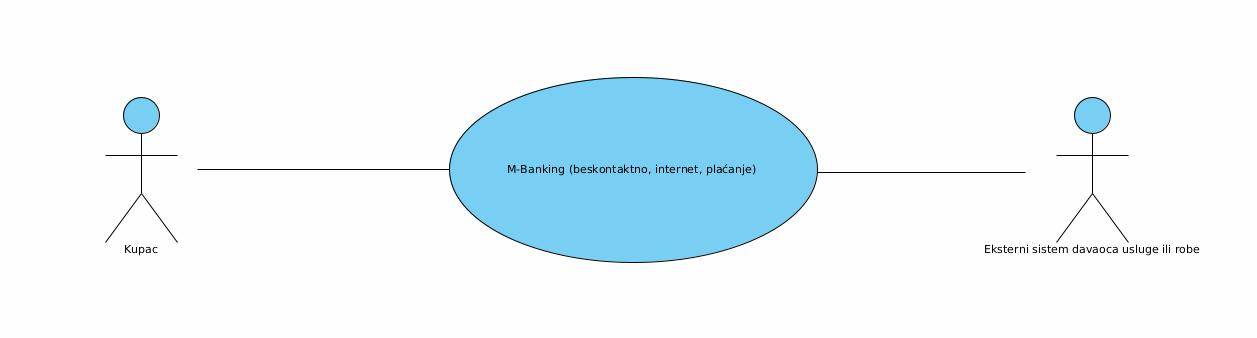
\includegraphics[scale = 0.27]{./UseCases/Pictures/M-Banking.jpg}

\subsubsection{Transakcije na ATM-u}

\textbf{Slučaj upotrebe: Transakcije na ATM-u}
\begin{enumerate}
  \item \textbf{Kratak opis: }
  Vršenje transakcija i upita stanja na bankomatima (ATM uređajima)
  \item \textbf{Učesnici: }
    \begin{itemize}
        \item Korisnik bankarskih usluga, želi da izvrši transakciju ili upit stanja koristeći ATM za povezivanje na informacioni sistem banke.
     \end{itemize}
  \item \textbf{Preduslovi: }
    Korisnik bankarskih usluga mora imati aktivnu platnu karticu banke čijem informacionom sistemu se obraća.
  \item \textbf{Postuslovi: }
    Transakcija, ili upit stanja, je uspešno izvršena, Korisnik je uplatio/podigao željenu svotu novca i to je proknjiženo na informacionom sistemu, ili je korisnik dobio uvid u svoje stanje.
  \item \textbf{Osnovni tok: }
    \begin{enumerate}
      \item Korisnik se predstavlja informacionom sistemu pomoću platne kartice i PIN-a i bira jezik komunikacije
      \item Informacioni sistem proverava dobijene podatke
      \item Informacioni sistem nudi korisniku opcije koje je moguće izvršiti  
      \item Korisnik bira željenu akciju za izvršavanje
      \item U zavisnosti od izbora opcije, sistem prelazi u neki od sledećih koraka:  
      \begin{enumerate}
        \item Korisnik je izabrao opciju preuzimanja sredstava sa računa, sistem nastavlja sa radom u podtoku P1
        \item Korisnik je izabrao opciju uplate sredstava na račun, sistem nastavlja sa radom u podtoku P2
        \item Korisnik je izabrao opciju provere stanja na računu, sistem nastavlja sa radom u podtoku P3
      \end{enumerate}
      \item Informacioni sistem završava traženu akciju i nudi korisniku da mu stanje računa bude odštampano na računu 
      \item Korisnik bira opciju kojom govori sistemu da li želi papirnu priznanicu
      \item U zavisnosti od izbora opcije, sistem prelazi u neki od sledećih koraka:  
      \begin{enumerate}
        \item Korisnik je izabrao opciju štampanja papirne priznanice, sistem nastavlja sa radom u podtoku P4
        \item Korisnik je izabrao opciju preskakanja štampanja papirne priznanice, sistem bez podkoraka nastavlja sa radom
      \end{enumerate}
      \item Sistem prekida konekciju sa korišćenim ATM aparatom
    \end{enumerate}
  \item \textbf{Podtokovi: } 
    \item \begin{enumerate}
     
      \item Opcija preuzimanja sredstava sa računa (P1):
        
      \begin{enumerate}
          \item Informacioni sistem nudi korisniku prozor za unos željenih sredstava
          \item Korisnik unosi željeni iznos koji želi da preuzme
          \item Informacioni sistem proverava stanje na računu korisnika
          \item Informacioni sistem umanjuje stanje na računu za željeni iznos  
          \item Informacioni sistem, putem ATM aparata, isplaćuje korisniku željeni iznos
          \item Korisnik preuzima dobijeni iznos 
        \end{enumerate}
        
        \item Opcija uplate sredstava na račun (P2);
        
        \begin{enumerate}
          \item Informacioni sistem nudi korisniku prozor za unos koliko sredstava želi da uplati na račun
          \item Korisnik unosi željenu količinu sredstava koju želi da uplati
          \item Korisnik potvrđuje unos i prilaže sredstva na određeno mesto na ATM aparatu
          \item Informacioni sistem prima podatke i proverava da li se željeni unos poklapa sa stvarnim sredstvima
          \item Informacioni sistem povećava stanje na računu korisnika
        \end{enumerate}
     
        \item Opcija provere stanja računa (P3);
         
        \begin{enumerate}
          \item Informacioni sistem vrši proveru stanja na računu
          \item Informacioni sistem šalje korisniku informaciju o stanju na računu
          \item Korisnik potvrđuje da je video informaciju o stanju na računu
        \end{enumerate}
        
        \item Opcija štampanja stanja računa (P4);
         
        \begin{enumerate}
          \item Informacioni sistem vrši proveru stanja na računu
          \item Informacioni sistem putem ATM aparata štampa stanje na računu
          \item Korisnik preuzima odštampanu papirnu priznanicu
        \end{enumerate}
      \end{enumerate}
  \item \textbf{Alternativni tokovi: } 
  \begin{enumerate}
    \item \textbf{Informacioni istem banke primio nevalidne podatke:} Ukoliko sistem dobije nevalidne podatke u koraku a (broj kartice, PIN kod), sistem obaveštava korisnika putem ATM aparata i prekida komunikaciju.
    \item \textbf{Sistem banke primio potražnju veću nego što kupac može da izvrši: } Ukoliko korisnik želi da podigne sredstva koja nema na računu u koraku P1.ii, sistem obaveštava korisnika da to nije moguće odraditi i nudi mu da promeni iznos ili odustane od transakcije.
    \item \textbf{Sistem banke primio potražnju veću nego što ATM može da isporuči: } Ukoliko korisnik želi da podigne sredstva kojih nema u ATM aparatu P1.ii, sistem obaveštava korisnika da to nije moguće odraditi i nudi mu da promeni iznos ili odustane od transakcije.
    \item \textbf{Sistem banke dobio različite iznose: } Ukoliko korisnik unese veći unos za uplatu nego što je priložio sredstava P2.iii, sistem obaveštava korisnika, vraća mu sredstva i nudi mu da promeni unos ili odustane od transakcije.
    manjku sredstava i kupovina mu se poništava.
\end{enumerate}
  \item \textbf{Specijalni zahtevi: } ATM je u ispravnom stanju, za opciju uplate na račun, fizički je omogućena operacija.
  \item \textbf{Dodatne informacije: } /
\end{enumerate}


\subsubsection{M-Banking}

\textbf{Slučaj upotrebe: M-Banking} 
\newline
\textit{Zbog mnogo mogućnosti, opisane su samo neke od funkcionalnosti.}

\begin{enumerate}
  \item \textbf{Kratak opis: }
    Korišćenje usluga bankarskog sistema posredstvom m-banking aplikacije.
  \item \textbf{Učesnici: }
    \begin{itemize}
        \item Korisnik bankarskih usluga, želi da izvrši transakciju, proveri stanje računa, ima uvid u transakcije računa, bez odlaska do filijale ili bankomata.
     \end{itemize}
  \item \textbf{Preduslovi: }
    Korisnik bankarskih usluga mora imati aktiviranu mogućnost korišćenja m-banking aplikaciju kojom se obraća informacionom sistemu.
  \item \textbf{Postuslovi: }
    Korisnik je odradio željene akcije, stanje na računu je izmenjeno shodno izabranim akcijama. 
  \item \textbf{Osnovni tok: }
    \begin{enumerate}
      \item Korisnik se loguje na m-banking aplikaciju nekim od mogućih načina.
      \item Informacioni sistem proverava ispravnost primljenih podataka.
      \item Informacioni sistem nudi korisniku opcije koje je moguće izvršiti. 
      \item Korisnik bira željenu akciju za izvršavanje
      \item U zavisnosti od izbora opcije, sistem prelazi u neki od sledećih koraka:  
      \begin{enumerate}
        \item Korisnik je izabrao opciju "menjačnica" kojom sa jednog od svojih računa na drugi, pritom menjajući jednu valutu za drugu, sistem nastavlja sa radom u podtoku P1
        \item Korisnik je izabrao opciju pregleda transakcija, sistem nastavlja u podtoku P2.
      \end{enumerate}
      \item Informacioni sistem završava traženu akciju i nudi korisniku opcije kao iz koraka c. 
      \begin{enumerate}
        \item Korisnik može izabrati neku od ponuđenih opcija i tada idemo u korak d.
        \item Korisnik ne želi više da koristi aplikaciju i bira opciju za završetak korišćenja aplikacije, sistem nastavlja dalji rad po koracima.
      \end{enumerate}
      \item Sistem prekida konekciju, korisnik je izlogovan.
    \end{enumerate}
  \item \textbf{Podtokovi: } 
    \item \begin{enumerate}
     
      \item Opcija "menjačnica", prenos sa računa A na račun B, pritom računi nemaju istu valutu koja se skladišti (P1):
        
      \begin{enumerate}
          \item Informacioni sistem nudi korisniku prozor za unos sredstava koje želi da zameni u drugu valutu.
          \item Korisnik unosi željeni iznos koji želi da zameni
          \item Informacioni sistem proverava stanje na računu A 
          \item Informacioni sistem umanjuje stanje na računu A za željeni iznos  
          \item Informacioni sistem prebacuje iz valute računa A u valutu računa B
          \item Informacioni sistem povećava stanje na računu B za recipročni iznos
        \end{enumerate}
        
        \item Opcija pregleda transakcija (P2);
        
        \begin{enumerate}
          \item Informacioni sistem nudi korisniku prozor za unos filtera koje će se transakcije prikazati
          \item Korisnik unosi podatke za filter
          \item Korisnik potvrđuje podatke i prosleđuje ih informacionom sistemu
          \item Informacioni sistem prima podatke i proverava validnost istih
          \item Informacioni sistem filtrira transakcije po zadatom filteru
          \item Informacioni sistem prikazuje isfiltrirane transakcije korisniku
          \item Korisnik nakom pregleda transakcija, potvrđuje da je proverio željene transakcije
        \end{enumerate}

      \end{enumerate}
  \item \textbf{Alternativni tokovi: } 
  \begin{enumerate}
    \item \textbf{Informacioni istem banke primio nevalidne podatke:} Ukoliko sistem dobije nevalidne podatke u koraku a, korisnika obaveštava da je došlo do greške i ne dozvoljava mu da pristupi sistemu.
    \item \textbf{Sistem banke primio potražnju veću nego što kupac može da izvrši: } Ukoliko korisnik želi da prebaci sredstva koja nema na računu A u koraku P1.ii, sistem obaveštava korisnika da to nije moguće odraditi i nudi mu da promeni iznos ili odustane od transakcije.
    \item \textbf{Sistem banke nije dobio dozvolu za korišćenje lokacije: } Ukoliko korisnik ne dozvoli sistemu da koristi trenutnu lokaciju korisnika, sistem prikazuje sve filijale na nivou države.
\end{enumerate}
  \item \textbf{Specijalni zahtevi: } /.
  \item \textbf{Dodatne informacije: } /
\end{enumerate}

\end{document}
